\section{Integral}

Integral predstavlja površinu ispod grafa funkcije.

Moguće ga je definirati na nekoliko različitih načina, no najčešće se
primjenjuje Riemannova definicija zbog jednostavnosti, jer je bila prva dobro
definirana i jer je dovoljna za večinu jednostavnih primjena u fizici i
inženjerstvu.

\subsection{Definicija integrala}

\subsubsection{Riemannov integral}

\begin{definition}[Riemannov zbroj]
    Neka je $f: [a, b] \to \mathbb{R}$ funkcija definirana na zatvorenom
    intervalu $[a,b]$ u skupu realnih brojeva ($a,b: \mathbb{R}$).
    
    Neka je $P = (x_0, x_1, \dots, x_n)$ particija intervala $[a,b]$:
    $$
        a = x_0 < x_1 < x_2 < \dots < x_n = b
    $$

    \textbf{Riemannov zbroj} $S$ funckije $f$ na intevalu $[a,b]$ sa particijom
    $P$ je onda definiran kao
    $$
        S= \sum_{i=1}^n f(x_i^*) \Delta x_i\,,
    $$
    gdje je $\Delta x_i = x_i - x_{i-1}$, a $x_i^*\in[x_{i-1},x_i]$ bilo koji
    element u pripadnom podintervalu particije $P$.
\end{definition}

Veličina particija ne mora biti uniformna.

Ovisno o odabiru $x_i^*$, koji može biti i arbitrarno pozicioniran unutar
podintervala particije $P$.
Tako načinom odabira $x_i^*$ možemo dobiti različite vrste Riemannovih zbrojeva:
\begin{itemize}
    \item Ako je $x_i^* = x_{i-1}$ za svaki $i$, metodu integracije nazivamo \textbf{lijevo pravilo} i daje \textbf{lijevi Riemannov zbroj}.
    \item Ako je $x_i^* = x_i$ za svaki $i$, metoda je \textbf{desno pravilo} i daje \textbf{desni Riemannov zbroj}.
    \item Ako je $x_i^* = (x_i + x_{i-1})/2$ za svaki $i$, metoda je \textbf{pravilo srednje vrijednosti} i daje \textbf{srednji Riemannov zbroj}.
    \item Ako je $f(x_i^*) = \sup f([x_{i-1}, x_i])$ za svaki $i$, metoda je \textbf{gornje pravilo} i daje \textbf{gornji Riemannov zbroj}.
    \item Ako je $f(x_i^*) = \inf f([x_{i-1}, x_i])$ za svaki $i$, metoda je \textbf{donje pravilo} i daje \textbf{donji Riemannov zbroj}.
\end{itemize}

Kažemo da je funcija Riemann-integrabilna ako svi ti zbrojevi konvergiraju kako
veličina particija postaje finija (manja), tj. približava nuli. 

\begin{definition}[Riemannov integral]
    Riemannov integral funkcije $f$ postoji i jednak je $s$ ako za svaki
    $\varepsilon > 0$, postoji $\delta > 0$ takav da za bilo koju označenu
    particiju $x_0, \dots, x_n$, s točkama uzorkovanja $t_0, \dots, t_{n-1}$,
    čija norma (mesh) je manja od $\delta$ vrijedi:
    $$
        \left|\left( \sum_{i=0}^{n-1} f(t_i)(x_{i+1} - x_i) \right) - s\right| < \varepsilon
    $$
\end{definition}

S tom definicijom je teško raditi jer zahtjeva da razmatramo sve particije sa
određenim svojstvom (kojih može biti beskonačno mnogo), pa se u praksi
preferira:

\begin{definition}[Riemannov integral]
    Riemannov integral funkcije $f$ postoji i jednak je $s$ ako za svaki
    $\varepsilon > 0$, postoji označena particija $y_0, \dots, y_m$ sa točkama
    uzorkovanja $r_0, \dots, r_{m-1}$ takva da za svaku označenu particiju
    $x_0, \dots, x_n$ sa točkama uzorkovanja $t_0, \dots, t_{n-1}$, koja je uglađena
    od $y_0, \dots, y_m$ i $r_0, \dots, r_{m-1}$, vrijedi:
    $$
        \left|\left( \sum_{i=0}^{n-1} f(t_i)(x_{i+1} - x_i) \right) - s\right| < \varepsilon
    $$
\end{definition}

Nedostatak Riemannove definicije integrala je to što zahtjeva predznanje
rješenja kako bi se mogla dokazati integrabilnost funcije u mnogim slučajevima,
što nije moguće za neke generalne dokaze propozicija.

Drugi nedostatak je što za određivanje Riemannove sume, funkcija $f: [a, b] \to \mathbb{R}$
mora biti definirana za svaki $x \in [a, b]$, što nije uvijek slučaj.

\subsubsection{Darbouxov integral}

Darbouxov integral ima jednostavniju definiciju koja je ekvivalentna
Riemannovoj, zbog čega se često koristi kao uvod u Riemannovu definiciju.

Prethodno navedeni \textit{gornji Riemannov zbroj} i \textit{donji Riemannov
zbroj} se također nazivaju i \textbf{gornji Darbouxov zbroj} ($U_{f,P}$) i
\textbf{donji Darbouxov zbroj} ($L_{f,P}$), sukladno, jer se koriste u
Darbouxovoj definiciji integrala.

\begin{definition}[Darbouxov integral]
    Gornji Darbouxov integral funkcije $f$ je
    $$
        U_f = \inf\{U_{f,P}: P \text{ je particija } [a,b]\}
    $$

    Donji Darbouxov integral funkcije $f$ je
    $$
        L_f = \sup\{L_{f,P}: P \text{ je particija } [a,b]\}
    $$
\end{definition}

Funkcija je Darboux-integrabilna ako i samo ako je Riemann-integrabilna.

\subsubsection{Lebesgueov integral}

\begin{multicols}{2}
Lebesgueovog integrala je generalizacija Riemannovog integrala.

Ideja iza Lebesgueovog integrala je slična Riemannovom, samo se umjesto
particioniranja domene $[a,b]$ oslanja na particioniranje raspona funkcije $f$
za određene vrijednosti. Zbog toga je definicija fleksibilnija i daje očekivana
rješenja za funkcije koje nisu Riemman-integrabilne.

Primjer funkcije koja nije Riemman-integrabilna:
$$
f(x) = \begin{cases}
    1,& x \in \mathbb{Q}\\
    0,& \text{inače}
\end{cases}
$$

\vspace*{\stretch{1}}

\columnbreak

\raggedleft
\def\svgwidth{0.6\columnwidth}
\input{../figure/lebesgue_integral.pdf_tex}

\end{multicols}

\subsubsection{Henstock-Kurzweilov integral}

Henstock-Kurzweilov integral je generalizacija Lebesgueovog integrala.

\begin{multicols}{2}

\noindent
Ovaj integral je prvotno definirao Arnaud Denjoy (1912.) jer je želio integrirati funkcije poput:
$$
    f(x) = \frac{1}{x} \sin \left( \frac{1}{x^3} \right)\,.
$$

Jer funkcija ima singularnost u $x=0$, tj. vrijednost jako kaotično oscilira iz
pozitivne u negativnu za sve manji korak u $x$, nije moguće odrediti površinu
ispod krivulje za tu funciju za $x=0$.

Henstock-Kurzweilov integral uvodi koncept mjerila ($\delta$) koje se koristi za
particioniranje intervala. To dopušta da se dijelovi funkcije koji se ponašaju
kaotičnije particioniraju sa finijim (manjim) podintervalima kako bi se njihova
površina mogla preciznije odrediti.

U točkama u kojima funkcija nije definirana je mjerilo $\delta = 0$, pa je i
taj član zbroja jednak $0$. Drugim riječima, ignoriramo površinu ispod krivulje
za vrijednosti za koje ona nije definirana.

Tako "skoro sve" funkcije postaju integrabilne.

\columnbreak

\vspace*{\stretch{1}}
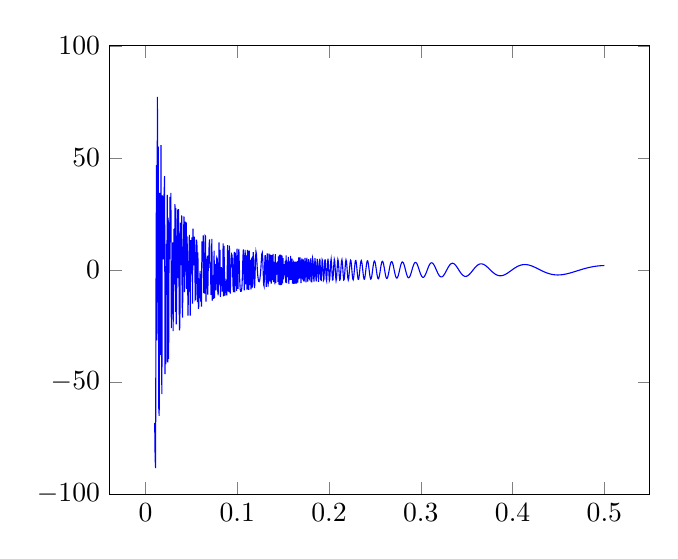
\begin{tikzpicture}
\begin{axis}[
    ymin=-100, ymax=100
]
    \addplot[domain=0.01:0.5,blue,samples=1000] {(1/x) * sin(deg(1/(x^3)))};
\end{axis}
\end{tikzpicture}
\vspace*{\stretch{1}}

\end{multicols}

\pagebreak

\subsection{Primitivna funkcija}
Neka je $f: \langle a, b \rangle \to \mathbb{R}$ funkcija.
\textbf{Primitivna funkcija} funkcije $f$ na $\langle a, b \rangle$ je svaka
funkcija $F: \langle a, b \rangle \to \mathbb{R}$ sa svojstvom:

$$
F'(x) = f(x),\quad\forall x \in \langle a, b \rangle.
$$

\begin{theorem}
    Neka je $f: \langle a, b \rangle \to \mathbb{R}$ funkcija, i $F$ i $G$
    bilo koje dvije primitivne funkcije od $f$ na $\langle a, b \rangle$. Tada
    postoji konstanta $C\in\mathbb{R}$ takva da vrijedi:

    $$
    F(x) = G(x) + C,\quad\forall x \in \langle a, b \rangle.
    $$
\end{theorem}

Za definiciju integrala je bitan \fancyeq[][lagrangeov teorem srednje vrijednosti]{thorem:lagrange}.

\begin{example}
    Odredi jednu primitivnu funkciju sljedećih funkcija:
    \begin{enumerate}
        \item $f(x) = \sin x$,
        \item $f(x) = e^x$,
        \item $f(x) = {\frac{1}{x}}$,
        \item $f(x) = {\frac{1}{\sqrt{x}}}$.
    \end{enumerate}
\end{example}

\begin{enumerate}
    \item $F(x) = \cos x$
\end{enumerate}

\begin{example}
    Odredi primitivnu funkciju $F(x)$ funkcije:
    $$
        f(x) = \begin{cases}
            2, & x < 0, \\
            e^x, & x \geq 0.
        \end{cases}
    $$

    koja je neprekidna i za koju vrijedi $F(-1) = 4$.
\end{example}

\begin{example}
    Dokaži da je $\displaystyle \phi(x)=\int_a^x f(x)\,dt$ primitivna funkcija neprekidne funkcije $f$ na intervalu $[a,b]$.
\end{example}

\subsection{Neodređeni integral}

\textbf{Neodređeni integral} funkcije $f$, s oznakom $\int f(x)\,dx$, je skup svih
primitivnih funkcija funkcije $f(x)$. Vrijedi:

$$
\int f(x)\,dx = \{F(x) + C\ |\ C\in\mathbb{R}\},
$$

pri čemu $F(x)$ označava primitivnu funkciju funkcije $f(x)$, a $C$ konstantu.

Prema tome su neodređeni integral i derivacija inverzne operacije te su povezane
sljedećim relacijama:

\begin{align*}
    \left(\int f(x)\,dx\right)' &= f(x),\\
    \int F'(x)\,dx &= F(x) + C.
\end{align*}

Derivacija integrala jednaka je podintegralnoj funkciji, odnosno integriranje
poništava deriviranje do na konstantu.

\subsection{Svojstva integrala}

\begin{proposition}[pravilo u umnošku s konstantom]
    $$
    \int{{k\,f\left( x \right)\,dx}} = k\int{{f\left( x \right)\,dx}}
    $$
\end{proposition}

Pretpostavimo da je $\mathrm{F}(x)$ antiderivacija funckije $f(x)$,
i da vrijedi $\mathrm{F}'(x) = f(x)$.

Onda možemo zapisati koristiti svojstva deriviranja kako bismo dobili:
$$
    (k\mathrm{F}(x))' = k \cdot \mathrm{F}'(x) = k \cdot f(x)
$$

\begin{proposition}[svojstvo linearnosti]
    Integral zbroja ili razlike funkcija $f(x)$ i $g(x)$ je jednak zbroju ili razlici dva integrala tih funckija:
    $$
    \int_a^b (\alpha f(x) + \beta g(x))\,dx = \alpha \int_a^b f(x)\,dx \pm \beta \int_a^b g(x)\,dx\,.
    $$
\end{proposition}


Pretpostavimo da je $F\left( x \right)$ antiderivacija $f\left( x \right)$,
i da je $\mathrm{G}\left( x \right)$ antiderivacija $g\left( x \right)$.

Dakle vrijedi $\mathrm{F}'\left( x \right) = f\left( x \right)$ i $\mathrm{G}'\left( x \right) =
g\left( x \right)$.

Osnovna svojstva o derivacijama nam također govore da vrijede slijedeće jednakosti:
\begin{itemize}
    \item $\left( \mathrm{F}\left( x \right) \pm \mathrm{G}\left( x
    \right) \right)' =
    \mathrm{F}'\left( x \right) \pm \mathrm{G}'\left( x \right) =
    f\left( x \right) \pm g\left( x \right)$,
    \begin{itemize}
        \item $F\left( x \right) + G\left( x \right)$ je antiderivacija izraza
        $f\left( x \right) + g\left( x \right)$,
        \item $F\left( x \right) - G\left( x
        \right)$ je antiderivacija izraza $f\left( x \right) - g\left( x \right)$.
    \end{itemize}
\end{itemize}

$$
\int{{f\left( x \right) \pm g\left( x \right)\,dx}} = F\left( x
\right) \pm G\left( x \right) + c = \int{{f\left( x \right)\,dx}} \pm
\int{{g\left( x \right)\,dx}}
$$


\subsection{Direktna integracija}

Budući da je neodređeni integral "\textit{antiderivacija}", čitanjem tablice
derivacija u obrnutom smjeru dobivamo tablicu integrala.

Iz svojstva linearnosti derivacije slijedi \textbf{svojstvo linearnosti}
neodređenog integrala:

$$
\int \left[af(x) + bg(x)\right]\,dx = a \int f(x)\,dx + b \int g(x)\,dx.
$$

\textbf{Direktna integracija} svodi se na primjenu tablice integrala i svojstva
linearnosti.

\begin{example}
    Izračunajte integral:

    \begin{enumerate}
        \item $\displaystyle \int \left(4 cos(x) + \frac{1}{2} x^3 - 3\right)$
    \end{enumerate}
\end{example}

\subsection{Metoda supstitucije}

\textbf{Metoda supstitucije}, također nazvana i \textbf{u-supstitucija} je
postupak u kojem se zamjenom stare varijable integracije novom, neodređeni
integral transformira u novi oblik. Primjenjuje se kada želimo integrirati neku
kompozicuju funkcija.

Izvodi se iz pravila za derivaciju kompozicije funkcija.

\bigskip
\noindent
Za primjenu metode supstitucije potreban je integral oblika:
$$
\int f[g(x)]\,g'(x)\,dx,
$$

\noindent
a primjenjujemo ju tako da:
\begin{enumerate}
    \item ako je potrebno, uređujemo funkciju kako bi mogli primjeniti metodu
    supstitucije,
    \item odabiremo novu varijablu integracije $u = g(x)$, pri čemu je $g(x)$
    derivabilna funkcija,
    \item određujemo $du = g'(x)\,dx$,
    \item zamjenom varijabli u integralu dobivamo novi integral u kojem je
    integrirana varijabla $u$, a koji je jednostavnijeg oblika: $\displaystyle
    \int f[g(x)]g'(x)\,dx = \int f(u)du,$
    \item rješavanjem tog integrala dobivamo: $\displaystyle \int f(u)du = F(u)
    + C$, te konačno,
    \item vraćamo se na staru varijablu integracije $x$: $F(u) + C = F[g(x)] +
    C.$
\end{enumerate}

\begin{example}
    Izračunajte integrale:
    \begin{enumerate}
        \item $\displaystyle \int \cos (5x)\,dx$,
        \item $\displaystyle \int \sqrt{2x + 3}\,dx$,
        \item $\displaystyle \int \frac{\ln x}{x}\,dx$,
        \item $\displaystyle \int (3x^2+2x)e^{x^3+x^2}\,dx$,
    \end{enumerate}
\end{example}

\begin{align*}
\int \cos 5x\,dx &= \begin{Bmatrix} u = 5x \\ du = (5x)'dx = 5\,dx \\ dx = \frac{du}{5} \end{Bmatrix} = \int \cos u\,du \\
                 &= \frac{1}{5}\sin u + C = \frac{1}{5}\sin 5x + C, \qquad C \in \mathbb{R}
\end{align*}
